%Preamble
\documentclass{article}
\usepackage{hyperref}
\usepackage[
    type={CC},
    modifier={by-nc-sa},
    version={3.0},
]{doclicense}
\usepackage[landscape]{geometry}
\usepackage{url}
\usepackage{multicol}
\usepackage{amsmath}
\usepackage{rotating}
\usepackage{dsfont}
\usepackage{esint}
\usepackage{amsfonts}
\usepackage{tikz}
\usetikzlibrary{decorations.pathmorphing}
\usepackage{amsmath,amssymb}
\usepackage{wasysym}

\usepackage{siunitx}

\usepackage{colortbl}
\usepackage{xcolor}
\usepackage{mathtools}
\usepackage{amsmath,amssymb}
\usepackage{enumitem}
\makeatletter

\newcommand*\bigcdot{\mathpalette\bigcdot@{.5}}
\newcommand*\bigcdot@[2]{\mathbin{\vcenter{\hbox{\scalebox{#2}{$\m@th#1\bullet$}}}}}
\makeatother

\title{ELEC 221 Final Formula Sheet}
\usepackage[english]{babel}
\usepackage[utf8]{inputenc}

\renewcommand{\baselinestretch}{1.15}

\advance\topmargin-.8in
\advance\textheight3in
\advance\textwidth3in
\advance\oddsidemargin-1.5in
\advance\evensidemargin-1.5in
\parindent0pt
\parskip2pt
\newcommand{\hr}{\centerline{\rule{3.5in}{1pt}}}
\newcommand\subtopic[1]{
    \textbf{#1}
    \vspace{.1cm}
    \hrule
    \vspace{.2cm}}

% custom commands
\newcommand{\ds}{\displaystyle}

\begin{document}

\begin{center}{\huge{\textbf{ELEC 221 Final Formula Sheet}}}\\
\end{center}
\begin{multicols*}{2}

\tikzstyle{mybox} = [draw=black, fill=white, very thick,
    rectangle, rounded corners, inner sep=10pt, inner ysep=10pt]
\tikzstyle{fancytitle} =[fill=black, text=white, font=\bfseries]

% change to make vertical spacing larger or smaller
\renewcommand{\arraystretch}{2.1}

%------------ CT ---------------
\begin{tikzpicture}
\node [mybox] (box){%
    \begin{minipage}{0.45\textwidth}
    \begin{tabular}{lp{8cm} l}
        Time domain convolution & $\ds y(t) = \int_{-\infty}^{\infty} x(\tau) h(t - \tau) d\tau$\\
        Fourier series & $\ds x(t) = \sum_{k=-\infty}^{\infty} c_{k} e^{jk\omega t}$\\
        Fourier coefficients & $\ds c_{k} =\frac{1}{T} \int_{T} x(t) e^{-jk\omega t}dt $\\
        Fourier transform & $\ds X(j\omega) =  \int_{-\infty}^{\infty} x(t)  e^{-j \omega t}dt$\\
        Inverse Fourier transform & $\ds x(t) = \frac{1}{2\pi}  \int_{-\infty}^{\infty}X(j\omega)   e^{j \omega t}d\omega$\\
        Laplace transform & $\ds X(s) =  \int_{-\infty}^{\infty} x(t) e^{-st} dt$\\
        Parseval's Identity & $\ds \frac{1}{T} \int_{T} |x(t)|^{2} dt = \sum_{k=-\infty}^{\infty} |c_{k}|^{2}$\\
        Group delay & $\ds \tau(\omega) = -\frac{d}{d\omega} \left( \varangle H(j\omega) \right)$\\
        Differential equations & $\ds \sum_{k=0}^{N} a_{k} \frac{d^{k}y(t)}{dt} = \sum_{k=0}^{M} b_{k} \frac{d^{k}x(t)}{dt}$\\
        Derivative identity & for $\ds x(t) \xleftrightarrow{\mathcal{F}} X(j\omega), \enskip \ds \frac{dx(t)}{dt}\xleftrightarrow{\mathcal{F}} j\omega X(j\omega)$\\
         & for  $\ds x(t) \xleftrightarrow{\mathcal{L}} X(s), \enskip \ds \frac{dx(t)}{dt}\xleftrightarrow{\mathcal{F}} s X(s)$\\
        Step response & $\ds s(t) = h(t) * u(t) = \int_{-\infty}^{t} h(\tau) d\tau$\\
        General form of 2nd order ODE & $\ds \frac{d^{2}y(t)}{dt^{2}} + 2\zeta \omega_{n} \frac{dy(t)}{dt} + \omega_{n}^{2}
  y(t) = \omega_{n}^{2} x(t)$
    \end{tabular}
    \end{minipage}
};
%------------ CT ---------------------
\node[fancytitle, right=10pt] at (box.north west) {Continuous Time};
\end{tikzpicture}



%------------ General Identities ---------------
\begin{tikzpicture}
\node [mybox] (box){%
    \begin{minipage}{0.8\textwidth}
    \begin{tabular}{lp{4cm} l lp{4cm}}
        Euler's Identity & $\ds e^{j\theta} = \cos\theta + j \sin \theta$ & Quadratic formula $\quad ax^2 + bx + c = 0 \quad x = \frac{1}{2a}\left(-b  \pm \sqrt{b^2 - 4ac} \right) $\\
        Geometric series & $\ds \sum_{k=0}^{N} z^{k} = \frac{1 - z^{N+1}}{1 - z}$& Integration by parts  $\quad \int_a^b u dv = u v |^b_a - \int_a^b v du$ \\
        & $\ds \sum_{k=0}^{N-1}e^{\frac{2 \pi j k}{N}} = 0$ 
    \end{tabular}
    \end{minipage}
};
%------------ General Identities ---------------------
\node[fancytitle, right=10pt] at (box.north west) {General Identities};
\end{tikzpicture}



%------------ DT ---------------
\begin{tikzpicture}
\node [mybox] (box){%
    \begin{minipage}{0.45\textwidth}
    \begin{tabular}{lp{8cm} l}
        Time domain convolution & $\ds y[n] =
        \sum_{k=-\infty}^{\infty} x[k] h[n - k]$\\
        Discrete Fourier series & $\ds x[n] = \sum_{k=0}^{N-1} c_{k} e^{jk\frac{2\pi}{N} n}$\\
        Fourier coefficients & $\ds c_{k} =\frac{1}{N} \sum_{n=0}^{N-1} x[n] e^{-jk\frac{2\pi}{N} n}$\\
        Discrete Fourier transform & $\ds X(e^{j\omega}) =  \sum_{n=-\infty}^{\infty} x[n]  e^{-j \omega n}$\\
        Inverse discrete Fourier transform & $\ds x[n] =  \frac{1}{2\pi} \int_{2\pi} X(e^{j\omega}) e^{j \omega n} d\omega$\\
        Z-transform & $\ds X(z) =  \sum_{n=-\infty}^{\infty} x[n] z^{-n}$\\
        Parseval's Identity & $\ds \frac{1}{N}\sum_{n=0}^{N-1} |x[n]|^{2} = \sum_{k=0}^{N-1} |c_{k}|^{2}$\\
        Group delay & $\ds \tau(\omega) = -\frac{d}{d\omega} \left( \varangle H(e^{j\omega}) \right)$\\
        Difference equation & $\ds \sum_{k=0}^{N} a_{k} y[n-k] = \sum_{k=0}^{M} b_{k} x[n-k]$\\
        Time shift identity & for where $\ds x[n] \xleftrightarrow{\mathcal{F}} X(e^{j\omega})$\\
         & $\ds x[n-k]\xleftrightarrow{\mathcal{F}} e^{-jk\omega} X(e^{j\omega})$\\
        Frequency shift identity &  $e^{j\omega_0 n} x[n]\xleftrightarrow{\mathcal{F}} X(e^{j(\omega - \omega_0)})$
    \end{tabular}
    \end{minipage}
};
%------------ DT ---------------------
\node[fancytitle, right=10pt] at (box.north west) {Discrete Time};
\end{tikzpicture}


\end{multicols*}

\newpage

\begin{sidewaysfigure}
    \centering
    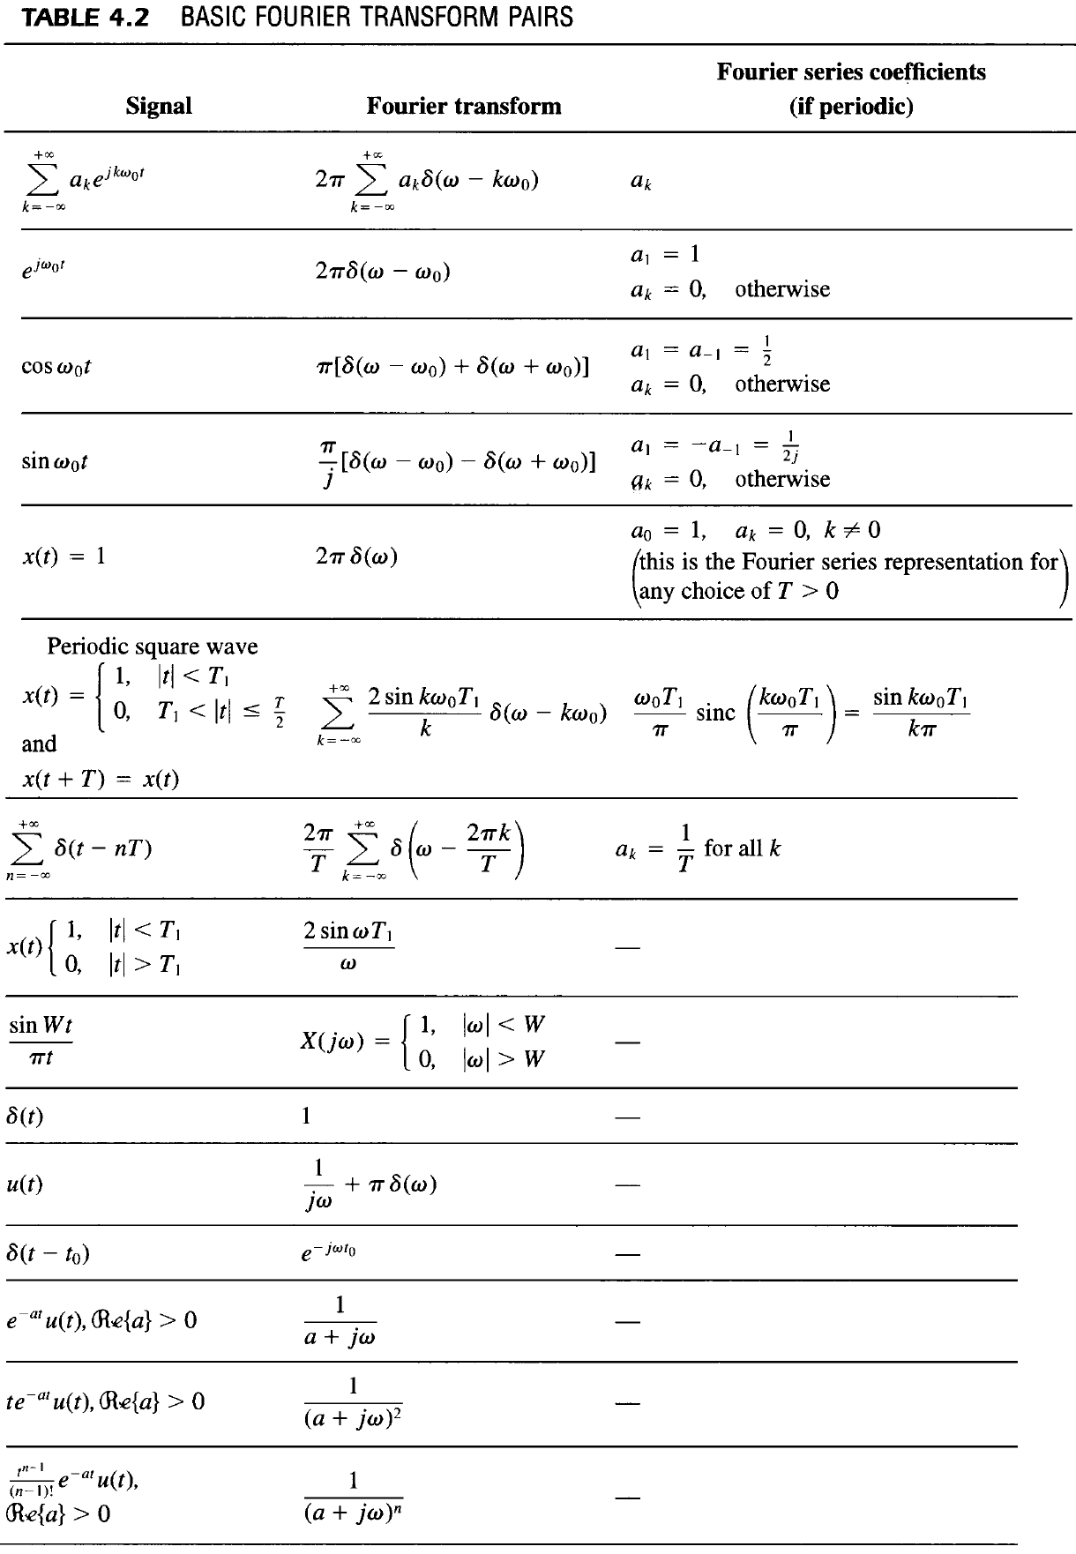
\includegraphics[height=\textheight]{table42-updated.png}
\end{sidewaysfigure}

\begin{sidewaysfigure}
    \centering
    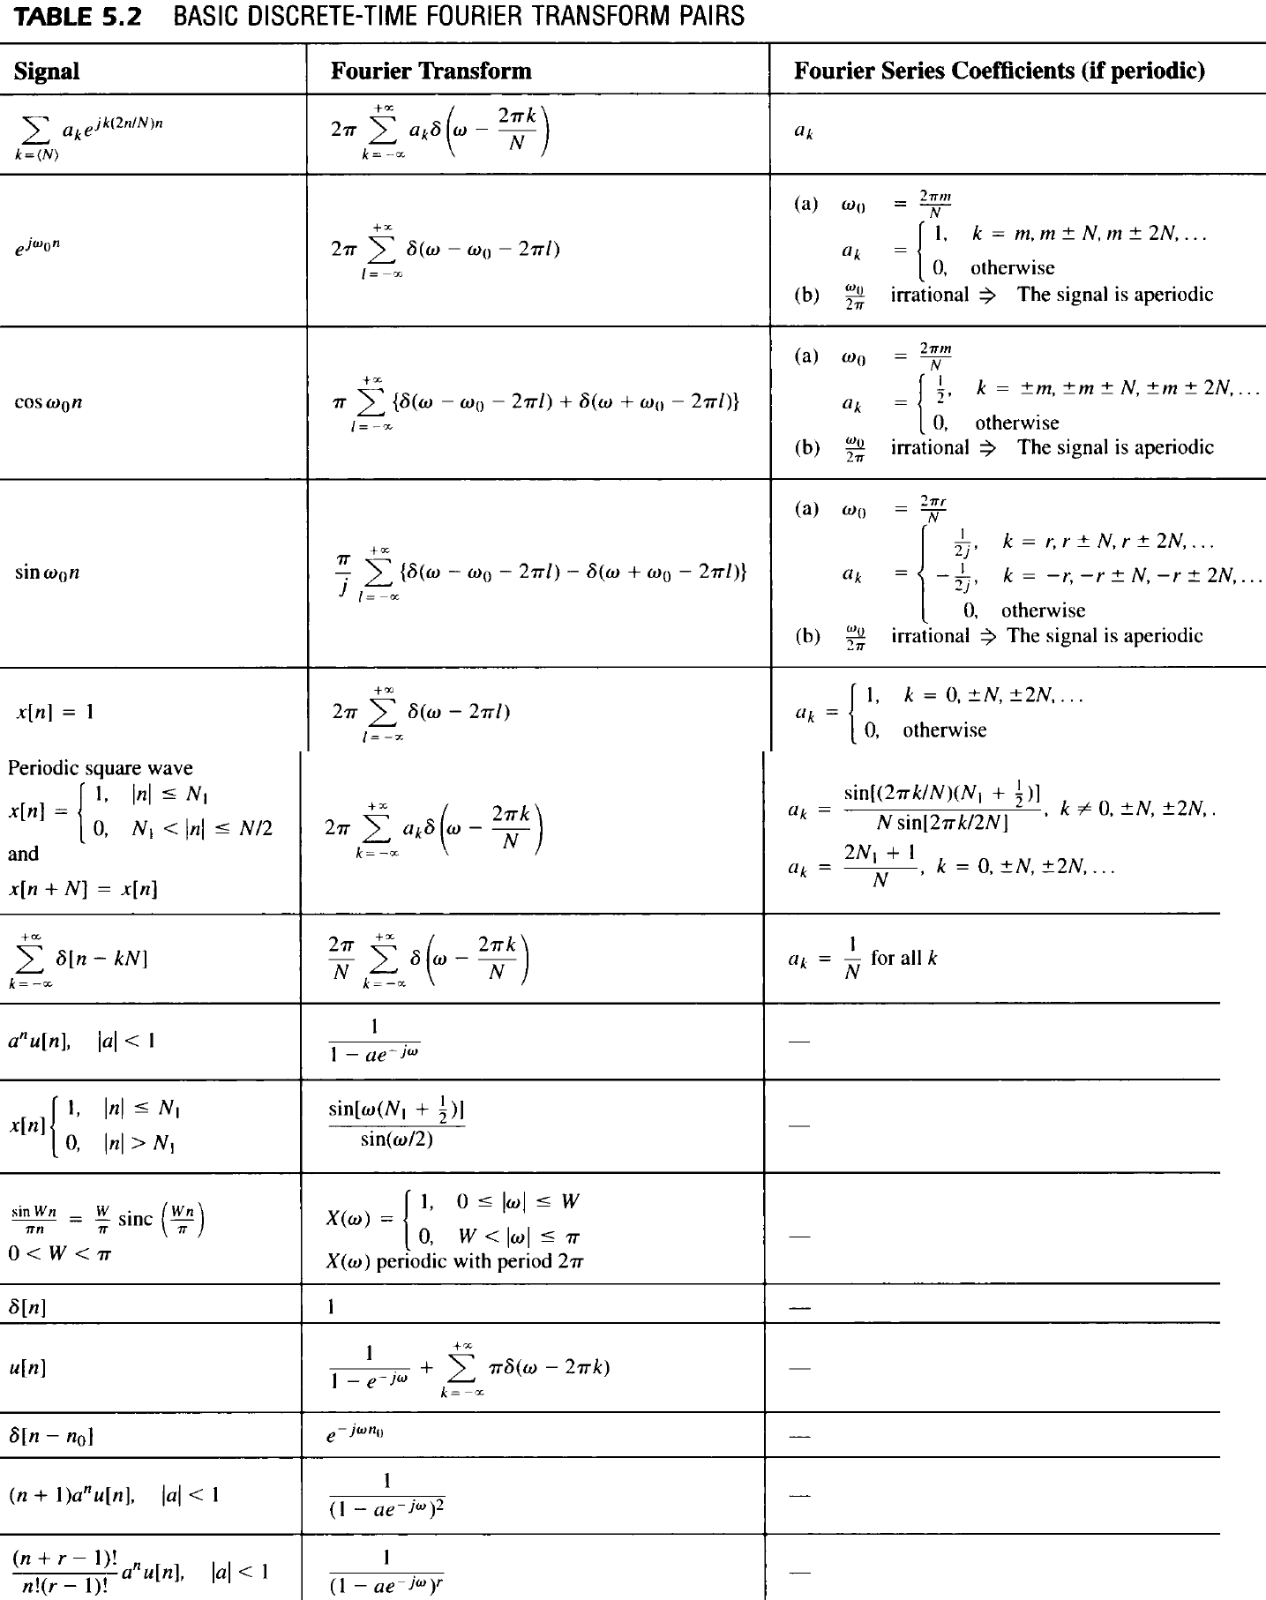
\includegraphics[height=\textheight]{table52-updated.png}
\end{sidewaysfigure}

\begin{sidewaysfigure}
    \centering
    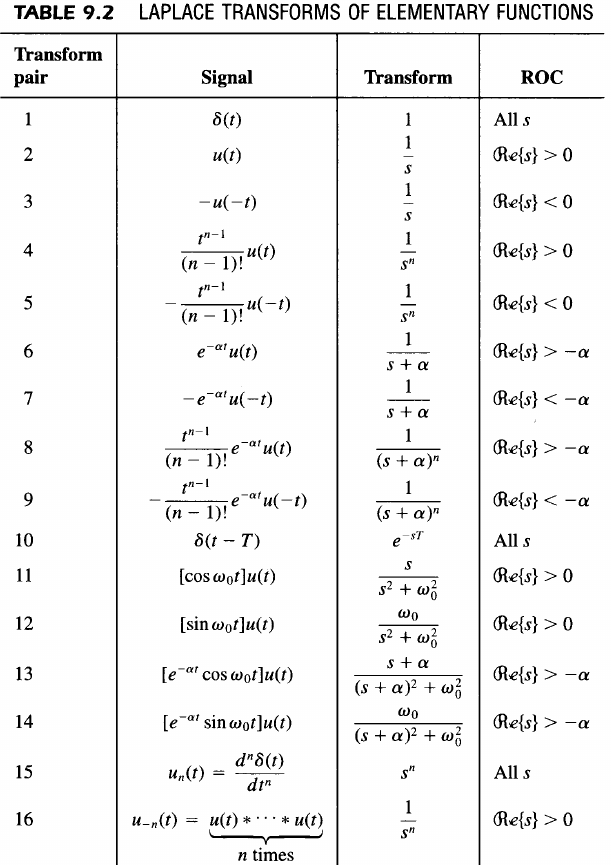
\includegraphics{table92.png}
\end{sidewaysfigure}

\begin{sidewaysfigure}
    \centering
    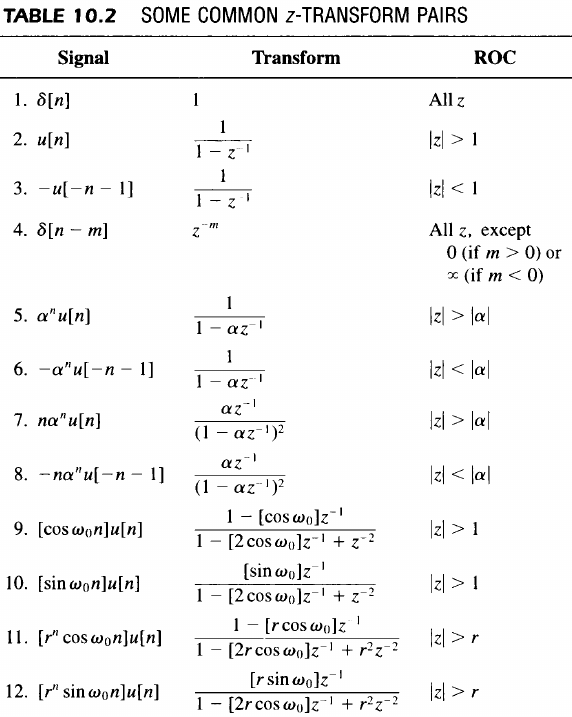
\includegraphics{table102.png}
\end{sidewaysfigure}

\end{document}